% !TEX root = ../Main.tex
\chapter{补形法：长方体模型}

某些三棱锥\textbf{天生"嵌在长方体里"}——把它"补"成长方体后，外接球即长方体的外接球，球心在长方体中心、半径为空间对角线之半。这一策略\textbf{避开繁琐的球心坐标计算}，一步到位。

\section{对棱相等的三棱锥}

\state{对棱相等三棱锥 $\to$ 长方体}{
    若三棱锥的\textbf{三组对棱两两相等}（设对棱长分别为 $a, b, c$——即 $AB = CD = a$，$AC = BD = b$，$AD = BC = c$），则可把它嵌入一个长方体中，使\textbf{三棱锥的六条棱成为长方体的六条面对角线}。

    设长方体棱长为 $m, n, p$，由面对角线关系：
    \[
    \begin{cases} m^2 + p^2 = a^2 \\ m^2 + n^2 = b^2 \\ n^2 + p^2 = c^2 \end{cases} \implies m^2 + n^2 + p^2 = \frac{a^2 + b^2 + c^2}{2}.
    \]
    长方体空间对角线 $= \sqrt{m^2 + n^2 + p^2}$，等于外接球直径 $2R$：
    \[
    (2R)^2 = m^2 + n^2 + p^2 = \frac{a^2 + b^2 + c^2}{2} \implies \boxed{R^2 = \frac{a^2 + b^2 + c^2}{8}.}
    \]
}

\begin{center}
\begin{tikzpicture}[scale=0.8]
    % Cuboid
    \draw[thick] (0,0,0) -- (4,0,0) -- (4,0,2) -- (0,0,2) -- cycle;
    \draw[thick] (0,3,0) -- (4,3,0) -- (4,3,2) -- (0,3,2) -- cycle;
    \draw[thick] (0,0,0) -- (0,3,0);
    \draw[thick] (4,0,0) -- (4,3,0);
    \draw[thick] (0,0,2) -- (0,3,2);
    \draw[thick] (4,0,2) -- (4,3,2);
    % The inscribed tetrahedron (4 alternate vertices)
    \coordinate (V1) at (0,0,0);
    \coordinate (V2) at (4,3,0);
    \coordinate (V3) at (4,0,2);
    \coordinate (V4) at (0,3,2);
    \draw[thick, red] (V1) -- (V2);
    \draw[thick, red] (V1) -- (V3);
    \draw[thick, red] (V1) -- (V4);
    \draw[thick, red] (V2) -- (V3);
    \draw[thick, red] (V2) -- (V4);
    \draw[thick, red] (V3) -- (V4);
    \node at (2, -0.8) {\small 嵌入长方体的"对棱相等"三棱锥：六棱即六条面对角线};
\end{tikzpicture}
\end{center}

\ex[对棱相等公式应用]{
    三棱锥 $ABCD$ 中 $AB = CD = \sqrt 5$，$AC = BD = \sqrt{10}$，$AD = BC = \sqrt{13}$。求其外接球半径。
}

\sol{
    $a = \sqrt 5, b = \sqrt{10}, c = \sqrt{13}$。
    \[
    R^2 = \frac{5 + 10 + 13}{8} = \frac{28}{8} = \frac{7}{2}, \qquad R = \sqrt{\frac{7}{2}} = \frac{\sqrt{14}}{2}.
    \]
    表面积 $= 4\pi R^2 = 14\pi$。
}

\section{墙角三棱锥（三条棱两两垂直）}

\state{墙角模型 $\to$ 长方体}{
    \textbf{墙角三棱锥}：一个顶点 $P$ 处有\textbf{三条棱 $PA, PB, PC$ 两两互相垂直}（像墙角一样）。这个三棱锥恰好是"长方体切去一角"——可以把它补回一个\textbf{长方体}，$P$-$ABC$ 就是长方体的一角，$PA, PB, PC$ 分别为长方体的三条棱。

    设 $PA = a, PB = b, PC = c$。长方体的空间对角线 $= \sqrt{a^2 + b^2 + c^2}$，即外接球的直径 $2R$：
    \[
    \boxed{R^2 = \frac{a^2 + b^2 + c^2}{4}.}
    \]
}

\begin{center}
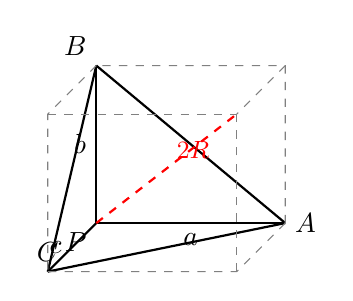
\begin{tikzpicture}[scale=0.8]
    \coordinate (P) at (0,0,0);
    \coordinate (A) at (3,0,0);
    \coordinate (B) at (0,2.5,0);
    \coordinate (C) at (0,0,2);
    \draw[thick] (P) -- (A) node[midway, below] {$a$};
    \draw[thick] (P) -- (B) node[midway, left] {$b$};
    \draw[thick] (P) -- (C) node[midway, left] {$c$};
    \draw[thick] (A) -- (B);
    \draw[thick] (A) -- (C);
    \draw[thick] (B) -- (C);
    % Complete cuboid
    \draw[dashed, gray] (A) -- (3,2.5,0) -- (B);
    \draw[dashed, gray] (A) -- (3,0,2) -- (C);
    \draw[dashed, gray] (B) -- (0,2.5,2) -- (C);
    \draw[dashed, gray] (3,2.5,0) -- (3,2.5,2);
    \draw[dashed, gray] (3,0,2) -- (3,2.5,2);
    \draw[dashed, gray] (0,2.5,2) -- (3,2.5,2);
    \draw[thick, red, dashed] (P) -- (3,2.5,2) node[midway, above right] {\small $2R$};
    \node at (P) [below left] {$P$};
    \node at (A) [right] {$A$};
    \node at (B) [above left] {$B$};
    \node at (C) [above] {$C$};
\end{tikzpicture}
\end{center}

\ex[墙角模型公式应用]{
    三棱锥 $S$-$ABC$ 中 $SA \perp SB$、$SB \perp SC$、$SC \perp SA$，且 $SA = 1, SB = 2, SC = 3$。求其外接球半径与表面积。
}

\sol{
    $R^2 = \dfrac{1 + 4 + 9}{4} = \dfrac{14}{4} = \dfrac{7}{2}$，$R = \dfrac{\sqrt{14}}{2}$。

    表面积 $= 4\pi R^2 = 14\pi$。
}

\section{墙角模型的"变体"：三面对角线为棱}

\state{以三面对角线为棱的三棱锥}{
    如果三棱锥的三条棱\textbf{长度是某长方体的三条面对角线}，即
    \[
    \begin{cases} m^2 = a^2 + b^2 \\ n^2 = b^2 + c^2 \\ p^2 = a^2 + c^2 \end{cases}
    \]
    则 $m^2 + n^2 + p^2 = 2(a^2 + b^2 + c^2)$，而 $(2R)^2 = a^2 + b^2 + c^2$（长方体空间对角线），故
    \[
    \boxed{R^2 = \frac{m^2 + n^2 + p^2}{8}.}
    \]
    \textbf{注意与对棱相等公式的差别}：对棱相等时 $R^2 = (a^2+b^2+c^2)/8$，这里的 $a,b,c$ 是三棱锥的\textbf{实际棱长}；而这里 $m,n,p$ 是\textbf{特殊几何描述}下的棱长。
}

\rmkb{
    \textbf{补形法的适用特征}——\textbf{识别"可补成长方体"的立体}：
    \begin{itemize}
        \item \textbf{对棱相等}的三棱锥（三组对棱长相等）$\Rightarrow$ 棱为\textbf{面对角线}；
        \item \textbf{墙角三棱锥}（三棱两两垂直）$\Rightarrow$ 棱为长方体\textbf{棱}；
        \item \textbf{三棱锥某面垂直于另一面且共一边}——常可补长方体的\textbf{半个}；
        \item \textbf{三棱锥嵌在正方体顶点}（如取正方体四个交错顶点得正四面体）——共享外接球。
    \end{itemize}

    \textbf{方法本质}：\textbf{用立体"外接于}长方体"的\textbf{对称性}，避免求球心坐标。
}
